\documentclass[11pt, letterpaper, twoside]{article}
\usepackage{risk_price_inference}
\usepackage{algorithm} 
\usepackage[backend=biber, autopunct=true, authordate, hyperref=true, doi=false,
isbn=false, url=false, eprint=false]{biblatex-chicago} 
\addbibresource{risk_price_inference.bib}

\author{Xu Cheng\thanks{University of Pennsylvania, The Perelman Center for Political Science and Economics, 133 South 36th Street, Philadelphia, PA 19104, \href{mailto:xucheng@upenn.edu}{xucheng@upenn.edu}} \and Eric Renault\thanks{Brown University, Department of Economics -- Box B, 64 Waterman Street, Providence, RI 02912, \href{mailto:eric_renault@brown.edu}{eric\_renault@brown.edu}} \and Paul Sangrey\thanks{University of Pennsylvania, The Perelman Center for Political Science and Economics, 133 South 36th Street, Philadelphia, PA 19104, \href{mailto:paul@sangrey.io}{paul@sangrey.io}}}

\title{Identification Robust Inference for Risk Prices in Structural Stochastic Volatility Models}

\date{\today}

\begin{document}

\begin{titlepage}


\maketitle
\thispagestyle{empty}
\addtocounter{page}{-1}

\begin{abstract} 

\singlespacing \noindent 
In structural stochastic volatility asset pricing models, changes in volatility affect risk premia through two channels: (1) the investor's willingness to bear high volatility in order to get high expected returns as measured by the market risk price, and (2) the investor’s direct aversion to changes in future volatility as measured by the volatility risk price. Disentangling these channels is difficult and poses a subtle identification problem that invalidates standard inference. We adopt the discrete-time exponentially affine model of \textcite{han2018leverage}, which links the identification of volatility risk price to the leverage effect. In particular, we develop a minimum distance criterion that links the market risk price, the volatility risk price, and the leverage effect to the well-behaved reduced-form parameters governing the return and volatility's joint distribution. The link functions are almost flat if the leverage effect is close to zero, making estimating the volatility risk price difficult. We apply the conditional quasi-likelihood ratio test \textcite{andrews2016conditional} develop in a nonlinear GMM framework to a minimum distance framework. The resulting conditional quasi-likelihood ratio test is uniformly valid. We invert this test to derive robust confidence sets that provide correct coverage for the risk prices regardless of the leverage effect's magnitude. 

\end{abstract} 

\medskip
\jelcodes{C12, C14, C38, C58, G12}

\medskip

\keywords{weak identification, robust inference, stochastic volatility, leverage, market risk premium, volatility risk premium, risk price, confidence set, asymptotic size}

\end{titlepage}

% \tableofcontents
\clearpage

\section{Introduction}

An important question in finance is how investors optimally trade off risk and return. Economic theories predict investors demand a higher return as compensation for bearing more risk. Hence, we should expect a positive relationship between the mean and volatility of returns. Some seminal early papers proposed a static trade-off between risk and expected return, most notably the capital asset pricing model (CAPM) of \textcites{sharpe1964capital,lintner1965security}. In practice, volatility varies over time. Consequently, a large strand of the recent literature examines the dynamic tradeoff between volatility and returns, including structural stochastic volatility models ( \textcites{bansal2014volatility, dewbecker2017price} ).  In these models, investors care not just about how an asset's returns co-move with the volatility but also care how they co-move with changes in volatility. 

In structural stochastic volatility models, changes in volatility affect risk premia through two channels: (1) the investor's willingness to tolerate high volatility in order to get high expected returns as measured by the market risk price, and (2) the investor’s direct aversion to changes in future volatility as measured by the volatility risk price. We adopt the discrete-time exponentially affine model of \textcite{han2018leverage}, where the market risk price and the volatility risk price are represented by two structural parameters. In this model,  \textcite{han2018leverage} establish the important result that the identification of the volatility risk price depends on a substantial leverage effect, which is the negative correlation between return and change in volatility. 

Although the leverage effect is theoretically less than zero, it is difficult to quantify empirically and its estimate usually is small \parencites{aitsahalia2013leverage}. When the leverage effect is mild, the data only provide limited amount of information about the volatility risk, compared to the finite-sample noise in the data. This low signal-to-noise ratio,  modeled by weak identification, invalidates standard inference based on the generalized method of moments (GMM) estimator, see \textcites{stock2000GMM,andrews2012estimation}.

We provide identification-robust confidence set (CS) for the structural parameters that measure the market risk price, the volatility risk price, and the leverage effect. 
The robust CS provides correct asymptotic coverage, uniformly over a large set of models that allow for any amount of leverage effect. This uniform validity is crucial for the CS to have good finite-sample coverage \parencites{mikusheva2007uniform, andrews2010applications}. In contrast, standard confidence sets based on the GMM estimator and its asymptotic normality does not have uniform validity in the presence of small leverage effect. This applies to all structural parameters because they are estimated simultaneously.


The robust inference is achieved in two-steps. First, we establish a minimum distance criterion using link functions between the structural parameter and a set of reduced-form parameters that determine the joint distribution of the return and volatility. The structural model implies that the link functions are zero when evaluated at the true values of the structural parameters and the reduced-form parameters. Identification and estimation of these reduced form parameters are standard and not affected by small leverage effect. However, the link function is almost flat in the structural parameter when the leverage effect is small, resulting in weak identification. Second, given this minimum distance criterion, we invert the conditional quasi-likelihood ratio (QLR) test by \textcite{andrews2016conditional} to construct a robust confidence set. The key feature of this test is that the flat link function is treated as an infinite dimensional nuisance parameter. The critical value is constructed by conditioning on a sufficient statistic for this nuisance parameter and it is shown to yield a valid test regardless of the nuisance parameter. \Textcite{andrews2016conditional} develop this test in a GMM framework. We show it works in the  minimum distance context here and provide conditions for its asymptotic validity. For practitioners, we provide a deatiled algorithm for the construction of this simulation-based robust confidence set.


Our paper relates to the empirical analysis of the effect of volatility on risk premia. As \textcite{lettau2010measuring} mention,  the evidence here is inconclusive. \textcites{bollerslev1988capital, harvey1989timevarying, ghysels2005there, bali2006there, ludvigson2007empirical} find a positive relationship, while \textcites{campbell1987stock, breen1989economic, pagan1991nonparametric, whitelaw1994time, brandt2004relationship} find a negative relationship. In addition, some papers use both a market risk factor and a variance risk factor to explain the risk premia dynamics, including \textcites{christoffersen2013capturing, feunou2014risk, dewbecker2017price}. A substantial positive variance risk premium is documented by \textcites{bollerslev2008risk, drechsler2011whats}. We contribute to this literature by providing a new way to do inference for the market risk price and the volatility risk price. This new CS not only allows for both effects but also takes into account the potential identification issue.


The weak identification issue studied in this paper is relevant in many economic applications, ranging from linear instrumental variable models \parencite{staiger1994instrumental} to nonlinear structural models \parencites{mavroeidis2014empirical, andrews2015maximum}. This is the first paper to study this issue in structural asset pricing models with stochastic volatility. The conditional inference approach is introduced to the linear instrumental variable model by \textcite{moreira2003conditional} and applied to the nonlinear GMM problem by \textcite{kleibergen2005testing}. \Textcite{andrews2016conditional} propose conditional inference for nonlinear GMM problems with infinitely dimensional nuisance parameter. This paper applies it to a minimum distance criterion and extends the scope of its application to a new type of asset pricing model.

The rest of the paper is organized as follows. \Cref{sec:model} provides the model and its parameterization. \Cref{sec:ilnk functions} provides model-implied restrictions and use them to derive the link function. \Cref{sec:robust inference} provides the asymptotic distribution of the reduced-form parameter and robust inference for the structural parameter. A detailed algorithm to construct the robust confidence set is given in \cref{sec:conditional QLR}. \Cref{sec:simulation} show that the method works well in simulation, and \Cref{sec:empirical} provides estimates of the risk prices in an empirical application. \Cref{sec:conclusion} concludes. Proofs are given in the appendix.

\section{The Model}\label{sec:model}

This section provides a parametric structural model with stochastic volatility, following \textcite{han2018leverage}. They extend the discrete-time exponentially-affine model of \textcite{darolles2006structural}, and their model is a natural discrete-time analog of the \textcite{heston1993closedform} model. We specify this model using a stochastic discount factor (SDF), also called the pricing kernel, and the physical measure, which gives the joint distribution of the return and volatility dynamics.\footnote{The risk-neutral measure is unobserved due to the lack of option data.} We first define the SDF and parameterize it as an exponential affine function with unknown parameters. Then we provide parametric distribution for the physical measure. 
  
Let $P_t$ be the price of the asset. Let $r_{t+1}=\log(P_{t+1}/P_t)-r_f$ denote the log excess return minus the risk-free rate and $\sigma^2_{t+1}$ denote its volatility. The observed data is $W_t=(r_t,\sigma^2_{t})$ for $t=1,\ldots,T$. 
Let $\F_t$ be the representative investor's information set at time $t$ . 

\subsection{Stochastic Discount Factor and Its Parameterization}\label{sec:deriving_sdf_functions}

The prices of all assets satisfy the following asset pricing equation in terms of the stochastic discount factor (SDF):
%
  \begin{equation}
    P_t = \E\left[M_{t,t+1} \exp\left(-r_f\right) P_{t+1} \mvert \F_t \right]. 
  \end{equation}
%
  Following the definition of $r_{t+1}$, the pricing equation implies that for all assets
%
\begin{equation}
1 = \E\left[M_{t,t+1} \exp\left(r_{t+1}\right) \mvert \F_t \right].
\end{equation}

We start by parameterizing the SDF by the exponential affine model. Let $\pi$ be the price of volatility risk and $\theta$ be the price of market risk. They are both considered as structural parameters.

\begin{defn}{Parameterize the Stochastic Discount Factor}
 \label{defn:SDF}
%
 \begin{equation}
    M_{t,t+1}(\pi, \theta) = \exp\left(m_{0} + m_1 \sigma_t^2 - \pi \sigma^2_{t+1} - \theta r_{t+1}\right). 
 \end{equation}
\end{defn}

Throughout we assume that the two risks that command nonzero prices are the market risk price and the volatility risk price. Consequently, we only use variation in the first two moments of the data to estimate these parameters. 

% If higher moments, such as skewness and kurtosis are also priced factors, as in \textcites{harvey2000conditional, conrad2012exante, chang2013market}, our model is misspecified. However, as we only use information 

\subsection{Parameterizing the Volatility and Return Dynamics}

Next, we parameterize the joint distribution of $\left\lbrace W_t:t=1,\ldots, T\right\rbrace $. 
Following \textcite{han2018leverage}, we make the following assumptions. First, the return $r_t$ and volatility $\sigma^2_t$ are first-order Markov. Second, there is no Granger-causality from the return to the volatility. Third, returns are independent across time given the volatility. We do allow $\sigma^2_{t}$ and $r_{t}$ to be contemporaneously correlated, as they are in the data. 
Under these assumptions, the volatility drives all of the dynamics of the process. The only relevant information in the information set $\F_{t}$ for time $t+1$-measurable variables is contained in $\sigma^2_t$. In general, $\sigma^2_t$, $\sigma^2_{t+1}$, and $r_{t+1}$ form a sufficient statistic for $\F_{t+1}$. 

We adopt the conditional autoregressive gamma process as in \textcite{gourieroux2006autoregressive, han2018leverage} for the volatility process. The model is parameterized in terms of the Laplace transform: 
%
\begin{equation}
    \E\left[\exp(-x \sigma^2_{t+1}) \mvert \F_{t}\right] = \exp\left(- A(x) \sigma^2_{t} - B(x)\right)
    \label{eqn:vol_laplace_transform}
\end{equation}
%
for all $x \in \R$. The function $A(x)$ and $B(x)$ are parameterized as follows.


\begin{defn}{Parameterize the Volatility Dynamics}
     \label{defn:physical_vol_dynamics}
     \begin{align}
        \label{defn:a_PP}
        A(x) &\coloneqq \frac{\rho x}{1 + c x}, \\
        \label{defn:b_PP}
        B(x) &\coloneqq \delta \log(1 + c x),
     \end{align}
with $\rho \in [0,1-\epsilon],$ $c > \epsilon$, $\delta > \epsilon$ for some $\epsilon > 0$.
\end{defn}

In this specification, $\rho$ is a persistence parameter, and $c$ and $\delta$ are scaling parameters. We can see this clearly in the following conditional mean and variance formulas for $\sigma^2_{t+1}$.

\begin{remark}[Volatilty Moment Conditions] 
 \label{remark:vol_moment_conditions}
    \begin{align}
        \E\left[\sigma^2_{t+1} \mvert \sigma^2_t \right] &= \rho \sigma^2_t + c \delta,\\
%   
        \Var\left[\sigma^2_{t+1} \mvert \sigma^2_t \right] &= 2 c \rho \sigma^2_t + c^2 \delta.
%   
    \end{align}
\end{remark}

All parameters are identified in these two moments conditions.

Next, we model the return dynamics. Similar to the volatility dynamics, the distribution of $r_t$ given $\sigma^2_{t+1}$ and $\sigma^2_{t}$ is specified in terms of the Laplace transform:
%
\begin{equation}
    \label{eqn:return_laplace_transform}
    \E\left[\exp(- x r_{t+1}) \mvert \F_{t}, \sigma^2_{t+1} \right] = \exp\left(- C(x) \sigma^2_{t+1} - D(x) \sigma^2_t - E(x)\right)
\end{equation}
%
for all $x \in \R$. The function $C(x)$, $D(x)$, and $E(x)$ are parameterized as follows such that the return has a conditional Gaussian distribution.

\begin{defn}{Parameterize the Return Dynamics}
    \label{defn:physical_return_dynamics}
    \begin{align}
        C(x) &\coloneqq \psi x - \frac{1 - \phi^2}{2} x^2,\\
        D(x) &\coloneqq \beta x, \\
        E(x) &\coloneqq \gamma x
    \end{align}
with $\phi \in [-1+\epsilon, 0]$ for some $\epsilon>0$.
\end{defn}

Under this specification, we have the following representation of the conditional mean and variance for $r_{t+1}$.

\begin{remark}[Return Moment Conditions] 
	\label{remark:return_moment_conditions}
	\begin{align}
		\label{eqn:rtn_cond_mean}
		\E\left[r_{t+1} \mvert \sigma^2_t, \sigma^2_{t+1}\right] = \psi \sigma^2_{t+1} + \beta \sigma^2_t + \gamma, \\
		%   
		\label{eqn:rtn_cond_vol}
		\Var\left[r_{t+1} \mvert \sigma^2_t, \sigma^2_{t+1}\right] = (1 - \phi^2) \sigma^2_{t+1}.
		%   
	\end{align}
\end{remark}


The parameter $\phi$ represents the leverage effect because it measures the return volatility reduction after conditioning on the volatility path. All parameters are identified in these moment conditions. 

\section{Link Functions}\label{sec:ilnk functions}

So far, we have introduced the following parameters: $(m_{0},m_{1},\theta ,\pi )$ in SDF, $(\rho ,c,\delta )$ in the volatility dynamic, and $(\psi ,\beta ,\gamma ,\phi )$ in the return dynamic. Next, we explore restrictions among these parameters that are consistent with this model. In other words, not all of these parameters can change freely under the structural model.

We use these restrictions to construct link functions between a set of reduced-form parameters and a set of structural parameters. These link functions play an important role on separating the regularly behaved reduced-form parameters from the structural parameters. They also are used to conduct identification robust inference for the structural parameters based on a minimum distance criterion.
All of these restrictions are also imposed in the GMM estimation in \textcite{han2018leverage}. However, because the volatility risk price is weakly identified, they calibrate it instead of estimating it. Given this calibrated value, they proceed to esimate all other parameters with GMM. 

\subsection{Pricing Equation Restrictions}

We first explore restrictions implied by the pricing equation $\E[ M_{t,t+1}\exp (r_{t+1}) \ivert \F_{t}]=1$. We start wtih a simple result stating that the constants $m_{0}$ and $m_{1}$ are normalization constants implied by all the other parameters. Thus, $m_{0}$ and $m_{1}$ are not free parameters to be estimated. Instead, they should take the value given below, once other parameters are specified. These restrictions on $m_{0}$ and $m_{1}$ are obtained by applying the restriction $\mathbb{E[} M_{t,t+1}\exp (r_{t+1})|\mathcal{F}_{t}]=1$ to the risk free asset. Applying the same argument to any other asset, we also obtain another set of two restrictions, which can be written in terms of the coefficients $\beta $ and $ \gamma $ under the linear form of $D(x)$ and $E(x)$.

\begin{lemma}
    \label{Lemma m0 and m1}
    Given the parameterization in the model, the pricing equation $\E[M_{t,t+1}\exp (r_{t+1}) \ivert \F_{t}]=1$ implies that 
%
    \begin{align*}
        m_{0} &= E(\theta )+B\left( \pi +C\left( \theta \right) \right) , \\
%
        m_{1} &= D\left( \theta \right) +A\left( \pi +C\left( \theta \right) \right) ,
    \end{align*}
    %
    and
%
    \begin{align*}
        \gamma  &= B\left( \pi +C\left( \theta -1\right) \right) -B\left( \pi +C\left( \theta \right) \right), \\
        \beta  &= A\left( \pi +C\left( \theta -1\right) \right) -A\left( \pi +C\left( \theta \right) \right).
    \end{align*}
\end{lemma}

The two equalities on $\beta $ and $\gamma $ link them to the market risk price, $\theta$, and the volatility risk, $\pi$,  through the functions $A(\cdot),B(\cdot ),C(\cdot ),$ which also involve parameters $(\rho ,c,\delta ,\psi ,\phi ).$ We treat these two equalities as link functions in the minimum distance criterion specified below.

\subsection{Leverage Effect Restrictions}\label{sec:leverage effect restrict}


%In the data section, we will assume use a realized volatility measure as our measure of $\sigma^2_{t+1}$.
%In continuous time, we have the traditional \Ito\ isometry, i.e., abusing notation somewhat $\Var[r_{t+1} \ivert \sigma^2_t] = \E[\sigma^2_{t+1} \ivert \sigma^2_t]$.
%However, it does not hold in this context because of risk-premia and Jensen effects arising from  taking expectations of exponentially-affine functions. 



Following \textcite{han2018leverage}, we parameterize $\psi$ as 
%
\begin{equation}
    \label{eqn:leverage restriction}
    \psi \coloneqq k \phi + \frac{1 - \phi^2}{2} \sigma^2_{t+1} - (1-\phi^2) \theta \sigma^2_{t+1}
\end{equation}
%
for some constant $k$. The first part $k \phi$ is the leverage effect from the instantaneous correlation between $r_{t+1}$ and $\sigma^2_{t+1}$.
The second part is the traditional Jensen effect term that arises from taking expectation of a log-Gaussian random variable.  The third term arises from risk-aversion, which is proportional to $\theta$.
%By noting that 
% In particular, it measures the reduction in the return
% We first show that both parameter $\psi $ and $\phi $ are linked to the leverage effect. Given the variance of $r_{t+1}$ conditional on $(\sigma _{t+1}^{2},\sigma _{t}^{2}),$ specified in \cref{eqn:rtn_cond_vol}, we have
% %
% \begin{equation*}
%     \phi ^{2}=\sigma _{t+1}^{2}-\Var[r_{t+1}|\sigma _{t+1}^{2},\sigma _{t}^{2}].
% \end{equation*}
% %
% This shows that $\phi $ is linked to the leverage effect because it measures the return volatility reduction after conditioning on the volatility path.  On the other hand, given the mean of $r_{t+1}$ conditional on $(\sigma _{t+1}^{2},\sigma _{t}^{2}),$ specified in \cref{eqn:rtn_cond_mean}, we have\footnote{To see this result, note that the mean of $r_{t+1}-\psi \sigma _{t+1}^{2}$ given $(\sigma _{t+1}^{2},\sigma _{t}^{2})$ does not depend on $\sigma
% _{t+1}^{2}$.}
%
%\begin{equation}
%    \E[r_{t+1}|\sigma _{t+1}^{2},\sigma _{t}^{2}]-E[r_{t+1}|\sigma _{t}^{2}]=\psi \left \{ \sigma _{t+1}^{2}-E[\sigma _{t+1}^{2}|\sigma _{t}^{2}]\right \},
%    \label{eqn:vol_versus_psi}
%\end{equation}
%%
%we can solve for $k$ using our parametric model, assuming it is time-invariant.
In addition, \textcite{han2018leverage} show that $k$ is the value under which $\mathbb{C}\mathrm{orr}[r_{t+1},\sigma _{t+1}^{2}|\sigma _{t}^{2}]=\phi $ if this correlation is indeed time invariant. Guided by this condition, they show that $k=1/(2c)^{1/2}$ should be used for the volatility dynamic specified in \cref{eqn:vol_versus_psi}  and \cref{eqn:leverage restriction}.


\subsection{Structural and Reduced-Form Parameters}

Because $\phi$ is the leverage effect parameter, we group it together with market risk price $\theta$ and the volatility risk price $\pi $ and call $ \lambda =(\theta ,\pi ,\phi )^{\prime }$ structural parameters. These structural parameters are estimated by restrictions from this structural model. In contrast, the other parameters in the conditional mean and variance of the return and volatility, see \cref{remark:vol_moment_conditions} and \cref{remark:return_moment_conditions}, are simply estimated using these moments, without any model restrictions. As such, we call them the reduced-form parameters. Because $1-\phi ^{2}$ shows up in the conditional variance of $r_{t+1},$ see \cref{eqn:rtn_cond_vol}, we define $\zeta =1-\phi ^{2}$ as a reduced-form parameter and link it to the structural parameter $\phi$ through this relationship. To sum up, the reduced-form parameters are $\omega =(\rho ,c,\delta ,\psi ,\beta ,\gamma ,\zeta )^{\prime }.$

Using $\zeta $ as a reduced-form parameter has the additional benefit of avoiding the estimation of $\psi$ directly. Estimating $\phi $ when its true value is close to 0 results in an estimator with a non-standard asymptotic distribution due to the boundary constraint. The inference procedure below does not require estimation of $\phi$ and is uniform over $\phi$ even if its true value is on or close to the boundary $0$.

The link functions between the structural parameter $\lambda $ and the reduced-form parameter $\omega $ are collected together in
%
\begin{equation}
   g(\lambda, \omega) = 
%
    \begin{pmatrix}
        \gamma - [B\left( \pi +C\left( \theta -1\right) \right) -B\left( \pi +C\left( \theta \right) \right)] \\ 
        \beta - [A\left( \pi +C\left( \theta -1\right) \right) -A\left( \pi +C\left( \theta \right) \right)] \\ 
        \psi -(1-\phi ^{2})\theta +\frac{1}{2}(1-\phi ^{2})-1/(2c)^{1/2}\phi  \\ \zeta -\left( 1-\phi ^{2}\right) 
    \end{pmatrix}.
\end{equation}%
%
For the inference problem studied below, we know $g(\lambda _{0},\omega_{0})=0$ when evaluated at the true value of $\lambda $ and $\omega .$

\subsection{Identification}

One of the important contributions of \textcite{han2018leverage} is to establish the relationship between the identification of the volatility risk price and the leverage effect. In particular, they show that when the leverage effect parameter $\phi =0,$ the volatility risk price $\pi $ is not identified. To see this result, note that the only source of identification information on $\pi $ are the first two link functions in $g(\lambda _{0},\omega _{0})=0$, 
which come from \cref{Lemma m0 and m1}. Clearly, these two equations are independent of $\pi$ if $C(\theta )=C(\theta -1)$. Of course, general, there is no reason to assume that this is the case. Using the definition of $C(\cdot)$ and \cref{eqn:leverage restriction}, we have 
%
\begin{equation*}
    C(\theta )-C(\theta -1)=\psi -(1-\phi ^{2})\left( \theta -\frac{1}{2}\right) = k \phi.
\end{equation*}
%
Clearly, the strength of identification is governed by the strength of the leverage effect.
In other words, we need $\phi \neq 0$ to identify the volatility risk price $\pi$.

Even if $\phi \neq 0$, we do not know it. In practice, with a finite-sample size and different types of noise in the data, such as measurement errors and omitted variables, a much more substantial leverage effect is required to obtain a standard identification situation where the noise in the data is negligible compared to the information to identify $\pi$. However, if only a small leverage effect is found, as in \textcites{bandi2012timevarying, aitsahalia2013leverage}, or the magnitude of the leverage effect is completely unknown, an identification robust procedure is needed to conduct inference in this problem. We provide such a procedure now.

\section{Robust Inference for Risk Prices}\label{sec:robust inference}

\subsection{Asymptotic Distribution of the Reduced-Form Parameter}

Write $\omega :=(\omega _{1},\omega _{2},\omega _{3})^{\prime },$ where $\omega _{1}=(\rho ,c,\delta )\in O_{1},$ $\omega _{2}=(\gamma ,\beta ,\psi) \in O_{2}$, and $\omega _{3}=\zeta \in O_{3}.$ The parameter space for $ \omega $ is $O=O_{1}\times O_{2}\times O_{3}\subset R^{d_{\omega }}$. The true value of $\omega $ is assumed to be in the interior of the parameter
space.

Below we describe the estimator $\widehat{\omega } \coloneqq (\widehat{\omega }_{1}, \widehat{\omega }_{2},\widehat{\omega }_{3})^{\prime }$ and provide its asymptotic distribution. We estimate these parameters separately because $\omega _{1}$ only shows up in the conditional mean and variance of $\sigma _{t+1}^{2}$, $\omega_{2}$ only shows up in the conditional mean of $r_{t+1}$, and $\omega _{3}$ only shows up in the conditional variance of $
r_{t+1}.$

We first estimate $\omega _{1}=(\rho ,c)$ based on the conditional mean and variance of $\sigma _{t+1}^{2}$, which can be equivalently written as 
%
\begin{align}
    E[\sigma _{t+1}^{2}|\sigma _{t}^{2}] &= A\text{ and }E[\sigma _{t+1}^{4}|\sigma _{t}^{2}]=B,\text{ where }  \nonumber \\
%
    A &= \rho \sigma _{t}^{2}+c\delta \text{ and }B=A^{2}+\left( 2c\rho \sigma _{t}^{2}+c^{2}\delta \right) .
\end{align}
%
Because the conditional mean of $\sigma _{t+1}^{2}$ and $\sigma _{t+1}^{4}$ are linear and quadratic functions, respectively, of the conditioning variable $\sigma _{t}^{2},$ without loss of efficiency, they can be transformed to the unconditional moments
%
\begin{equation}
    E[h_{t}(\omega _{10})]=0,\text{ where }h_{t}(\omega _{1})=[(1,\sigma _{t}^{2})\otimes (\sigma _{t+1}^{2}-A),(1,\sigma _{t}^{2},\sigma _{t}^{4})\otimes (\sigma _{t+1}^{4}-B)]^{\prime },
\end{equation}
%
and $\omega _{10}$ represents the true value of $\omega _{1}$. The two-step GMM estimator of $\omega _{1}$ is%
%
\begin{equation}
    \widehat{\omega }_{1}=\underset{\omega _{1}\in O_{1}}{\arg \min }\left( T^{-1}\sum_{t=1}^{T}h_{t}(\omega _{1})\right) ^{\prime }\widehat{V}_{1}\left( T^{-1}\sum_{t=1}^{T}h_{t}(\omega _{1})\right) ,
    \label{omega 1 est}
\end{equation}%
%
where $\widehat{V}_{1}$ is a consistent estimator of $V_{1}=\sum_{m=-\infty }^{\infty }\Cov[h_{t}(\omega _{10}),h_{t+m}(\omega _{10})].$

We estimate $\omega _{2}$ by the generalized least squares (GLS) estimator because the conditional mean of $r_{t+1}$ is a linear function of the conditioning variable $\sigma _{t}^{2}$ and $\sigma _{t+1}^{2}$ and the conditional variance is proportional to $\sigma _{t+1}^{2}.$ The GLS estimator of $\omega _{2}$ is
%
\begin{align}
    \widehat{\omega }_{2} &= \left( \sum_{t=1}^{T}x_{t}x_{t}^{\prime }\right) ^{-1}\sum_{t=1}^{T}x_{t}y_{t},\text{ where }  \notag \\ 
%
    x_{t} &= \sigma _{t+1}^{-1}(1,\sigma _{t}^{2},\sigma _{t+1}^{2})^{\prime } \text{ and }y_{t}=\sigma _{t+1}^{-1}r_{t+1}.  \label{omega 2 est}
\end{align}
%
We estimate $\omega _{3}$ by the sample variance estimator
%
\begin{equation}
    \widehat{\omega }_{3}=T^{-1}\sum_{t=1}^{T}\left( y_{t}-\widehat{y}_{t}\right) ^{2},\text{ where }\widehat{y}_{t}=x_{t}^{\prime }\widehat{ \omega }_{2}.  
    \label{omega 3 est}
\end{equation}

Let $P$ denote the distribution of the data \{W_{t}=(r_{t+1}, \sigma _{t+1}^{2}):t\geq 1\}$ and $\mathcal{P}$ denote the parameter space of $P$. Note that the true values of the structural parameter and the reduced-form parameters are all determined by $P.$ We allow $P$ to change with $T.$ For notational simplicity, the dependence on $P$ and $T$ is suppressed.

Let 
%
\begin{equation}
    f_{t}(\omega) = 
%
    \begin{pmatrix}
        h_{t}(\omega _{1}) \\ 
        x_{t}(y_{t}-x_{t}^{\prime }\omega _{2}) \\ 
        (y_{t}-x_{t}^{\prime }\omega _{2})^{2}%
    \end{pmatrix}
%
     \in R^{d_{f}}\text{ and } 
%
     V =\sum_{m=-\infty }^{\infty }\Cov\left[f_{t}(\omega _{0}),f_{t+m}(\omega _{0})\right].
\end{equation}
%
The estimator $\widehat{\omega }$ defined above is based on the first moment of $f_{t}(\omega ).$ Thus, the limiting distribution of $\widehat{\omega }$ relates to the limiting distribution of $T^{-1/2}\sum_{t=1}^{T}(f_{t}(\omega _{0})-\E[f_{t}(\omega _{0}))$ following from the central limit theorem. Furthermore, because $\omega _{1}$ is the GMM estimator based on some nonlinear moment conditions, we need uniform convergence of the sample moments and their derivatives to show the consistency and asymptotic normality of $\widehat{\omega }_{1}.$ These uniform convergence follows from the uniform law of large numbers. Because $\widehat{\omega }_{2}$ is a simple OLS estimator by regressing $y_{t}$ and $x_{t},$ we need the regressors to not exhibit multicollinearity. We make the necessary assumptions below. All of them are easily verifiable with weakly dependent time series data.

Let $\widehat{V}$ denote a heteroskedasticity and autocorrelation consistent (HAC) estimator of $V$. The estimator $\widehat{V}_{1}$ is a submatrix of $\widehat{V}$ associate with $V_{1}.$ Let $H_{t}(\omega _{1})=\partial h_{t}(\omega _{1})/\partial \omega _{1}^{\prime }.$

\begin{assumpR}
    \label{assump:R}
    The following conditions hold uniformly over $P\in \mathcal{P}$, for some fixed $0 < C < \infty$.
    
    \begin{enumerate}
        \item $T^{-1}\sum_{t=1}^{T}(h_{t}(\omega_{1})-\E[ h_{t}(\omega _{1}))\rightarrow _{p}0$ and $T^{-1}\sum_{t=1}^{T}(H_{t}(\omega _{1})-\E[H_{t}(\omega _{1})])\rightarrow _{p}0,$ $\E[H_{t}(\omega _{1})]$ is continuous in $\omega _{1},$ all uniformly over the parameter space of $\omega _{1}$.
    %
        \item $T^{-1}\sum_{t=1}^{T}(x_{t}x_{t}^{\prime }-\E[ x_{t}x_{t}^{\prime }{])\rightarrow }_{p}0.$
    %
        \item $V^{-1/2}\{T^{-1/2}(\sum_{t=1}^{T}f_{t}(\omega _{0})-\E[f_{t}(\omega _{0}){]\} \rightarrow }_{d}N(0,I)$ and $\widehat{V} -V\rightarrow _{p}0.$
    %
        \item $C^{-1}\leq \lambda _{\min }(A)\leq \lambda _{\max }(A)\leq C$ for $A=V,\E[H_{t}\left( \omega _{1,0}\right) ^{\prime }H_{t}\left( \omega _{1,0}\right) ]),\E[x_{t}x_{t}^{\prime }],\E[ z_{t}z_{t}^{\prime }],$ where $z_{t}=(1,\sigma _{t}^{2},\sigma _{t}^{4})^{\prime }.$
    %
    \end{enumerate}
\end{assumpR}


Let $H(\omega _{1})=\mathbb{E[}H_{t}(\omega _{1})]$ and $\overline{H}(\omega _{1})=T^{-1}\sum_{t=1}^{T}H_{t}(\omega _{1}).$ Define
%
\begin{align}
%
    \mathcal{B} &= \diag\{[H(\omega _{10})V_{1}^{-1}H(\omega _{10})]^{-1}H(\omega _{10})V_{1}^{-1},\mathbb{E[}x_{t}x_{t}^{\prime }]^{-1},1\},  \notag \\
%
    \widehat{\mathcal{B}} &= \diag\{[\overline{H}(\widehat{\omega }_{1})^{\prime } \widehat{V}_{1}^{-1}\overline{H}(\widehat{\omega }_{1})]^{-1}\overline{H}( \widehat{\omega }_{1})^{\prime }\widehat{V}_{1}^{-1},[T^{-1}
\sum_{t=1}^{T}x_{t}x_{t}^{\prime }]^{-1},1\}.  
%
    \label{Fhat}
\end{align}
%
The following lemma provides the asymptotic distribution of the reduced-form parameter and a consistent estimator of its asymptotic covariance. Note that we put the asymptotic covariance on the left side of the convergence to allow the distribution of the data to change with sample size $T$.

\begin{lemma}
\label{Lemma Reduce}
Suppose \Cref{assump:R} holds. The following results hold uniformly over $P\in \mathcal{P}$.

\begin{enumerate}
    \item $\xi _{T}:=\Omega ^{-1/2}T^{-1/2}(\widehat{\omega } -\omega _{0})\rightarrow _{d}\xi \sim N(0,I),$ where $\Omega =\mathcal{B}V \mathcal{B}^{\prime }.$

    \item $\widehat{\Omega }-\Omega \rightarrow _{p}0,$ where $\widehat{\Omega }=\widehat{\mathcal{B}}\widehat{V}\widehat{\mathcal{B}}^{\prime }.$
\end{enumerate}
\end{lemma}

\subsection{Weak Identification}

The true value of the structural parameter $\lambda$ and the reduced-form parameter $\omega$ satisfy the link function $g(\lambda _{0},\omega _{0})=0$. In a standard problem without any identification issues, we can estimate $\lambda _{0}$ by the minimum distance estimator, $\widehat{\lambda } =(\widehat{\theta },\widehat{\pi },\widehat{\phi })$, that minimizes $ Q_{T}(\lambda )=g(\lambda ,\widehat{\omega })^{\prime }W_{T}g(\lambda , \widehat{\omega })$ for some weighting matrix $W_{T}$ and construct tests and confidence sets for $\lambda _{0}$ using an asymptotically normal approximation for $T^{1/2}(\widehat{\lambda }-\lambda _{0})$. However, this standard method does not work in the present problem when $\pi _{0}$ is only weakly identified. In this case, $g(\lambda ,\widehat{\omega })$ is almost flat in $\pi $ and the minimum distance estimator of $\widehat{\pi }$ is not even consistent. To make the problem even more complicated, the inconsistency of $\widehat{\pi }$ has a spillover effect on $\widehat{\theta }$ and $\widehat{\phi },$ making the distribution of $\widehat{\theta }$ and $\widehat{\phi }$ non-normal even in large sample.

Before presenting the robust CS, we first introduce some useful quantities and provide some heuristic discussions of the identification problem and its consequence. Let $G(\lambda ,\omega )$ denote the partial derivative of $ g(\lambda ,\omega )$ with respect to (w.r.t.)\@ $\omega .$ Let $g_{0}(\lambda )=g(\lambda ,\omega _{0})$ and $G_{0}(\lambda )=G(\lambda ,\omega _{0})$ be the link function and its derivative evaluated at $\omega _{0}$ and $\widehat{g}(\lambda
)=g(\lambda ,\widehat{\omega })$ and $\widehat{G}(\lambda )=G(\lambda , \widehat{\omega })$ be the same quantities evaluated at the estimator $ \widehat{\omega }.$ The delta method gives 
%
\begin{equation}
    \eta _{T}(\lambda ):=T^{1/2}\left[ \widehat{g}(\lambda )-g_{0}(\lambda ) \right] =G_{0}(\lambda )\Omega ^{1/2}\cdot \xi _{T}+o_{p}(1),
    \label{emp pro}
\end{equation}
%
where $\xi _{T}\rightarrow _{d}N(0,I)$ following \cref{Lemma Reduce}.  Thus, $\eta _{T}(\cdot )$ weakly converges to a Gaussian process $\eta (\cdot )$ with covariance function $\Sigma (\lambda _{1},\lambda _{2})=G_{0}(\lambda _{1})\Omega G_{0}(\lambda _{2})^{\prime }.$

Following \cref{emp pro}, we can write $T^{1/2}\widehat{g}(\lambda )=\eta _{T}(\lambda )+T^{1/2}g_{0}(\lambda ),$ where $\eta _{T}(\lambda )$ is the noise from the reduced-form parameter estimation and $T^{1/2}g_{0}(\lambda )$ is the signal from the link function. Under weak identification, $ g_{0}(\lambda )$ is almost flat in $\lambda ,$ modeled by the signal $ T^{1/2}g_{0}(\lambda )$ being finite even for $\lambda \neq \lambda _{0}$ and $T\rightarrow \infty .$ Thus, the signal and the noise are of the same order of magnitude, yielding an inconsistent minimum distance estimator $ \widehat{\lambda }.$ This is in contrast with the strong identification scenario, where $T^{1/2}g_{0}(\lambda )\rightarrow \infty $ for $\lambda \neq \lambda _{0}$ as $T\rightarrow \infty $ and $g_{0}(\lambda _{0})=0.$ In this case, the signal is so strong that the minimum distance estimator is consistent.

The identification strength of $\lambda _{0}$ is determined by the function $ T^{1/2}g_{0}(\lambda ).$ However, this function is unknown and cannot be consistently estimated (due to $T^{1/2}$). Thus, we take the conditional inference procedure as in \textcite{andrews2016conditional} and view $ T^{1/2}g_{0}(\lambda )$ as an infinite dimensional nuisance parameter for the inference of $\lambda _{0}$. The goal is to construct robust CS for $\lambda _{0}$ that has correct size asymptotically regardless of this unknown nuisance parameter.

\subsection{Conditional QLR Test}\label{sec:conditional QLR}

We construct a CS for $\lambda $ by inverting the test $ H_{0}: \lambda =\lambda_{0}$ vs $H_{1}: \lambda \neq \lambda _{0}$. The test statistic is a QLR statistic that takes the form
%
\begin{equation}
    QLR(\lambda _{0}) \coloneqq T\widehat{g}(\lambda _{0})^{\prime }\widehat{\Sigma} (\lambda _{0},\lambda _{0})^{-1}\widehat{g}(\lambda _{0})-\underset{\lambda \in \Lambda }{\min }T\widehat{g}(\lambda )^{\prime }\widehat{\Sigma } (\lambda ,\lambda )^{-1}\widehat{g}(\lambda ),  
    \label{QLR stat}
\end{equation}
%
where $\widehat{\Sigma }(\lambda _{1},\lambda _{2},)=\widehat{G}(\lambda _{1})\widehat{\Omega }\widehat{G}(\lambda _{2})^{\prime }$ and $\widehat{ \Omega }$ is the consistent estimator of $\Omega $ defined above.

\Textcite{andrews2016conditional} provide the conditional QLR test in a nonlinear GMM problem, where $\widehat{g}(\lambda )$ is replaced by a sample moment. The same method can be applied to the present nonlinear minimum distance problem. Following \textcite{andrews2016conditional}, we first project $\widehat{g}(\lambda )$ onto $\widehat{g}(\lambda _{0})$ and construct a residual process
%
\begin{equation}
    \widehat{r}(\lambda )=\widehat{g}(\lambda )-\widehat{\Sigma }(\lambda ,\lambda _{0})\widehat{\Sigma }(\lambda _{0},\lambda _{0})^{-1}\widehat{g} (\lambda _{0}).  
    \label{red process}
\end{equation}
%
The limiting distribution of $\widehat{r}(\lambda )$ and $\widehat{g} (\lambda _{0})$ are Gaussian and independent. Thus, conditional on $\widehat{ r}(\lambda ),$ the asymptotic distribution of $\widehat{g}(\lambda )$ no longer depends on the nuisance parameter, $T^{1/2}g_{0}(\lambda ),$ making the procedure robust to all identification strength.

Specifically, we obtain the $1-\alpha $ conditional quantile of the QLR statistic, denoted by $c_{1-\alpha }(r,\lambda _{0}),$ as follows. For $ b=1,\ldots,B$, we take independent draws $\eta _{b}^{\ast }\sim N(0,\widehat{\Sigma }(\lambda _{0},\lambda _{0}))$ and produce a simulated process 
%
\begin{equation}
    g_{b}^{\ast }(\lambda ) \coloneqq \widehat{r}(\lambda )+\widehat{\Sigma }(\lambda ,\lambda _{0})\widehat{\Sigma }(\lambda _{0},\lambda _{0})^{-1}\eta _{b}^{\ast }
\end{equation}
%
and a simulated statistic
%
\begin{equation}
    QLR_{b}^{\ast }(\lambda _{0}) \coloneqq T\widehat{g}(\lambda _{0})^{\prime }\widehat{\Sigma }(\lambda _{0},\lambda _{0})^{-1}\widehat{g}(\lambda _{0})-\underset{\lambda \in \Pi }{\min }Tg_{b}^{\ast }(\lambda )^{\prime }\widehat{\Sigma } (\lambda ,\lambda )^{-1}g_{b}^{\ast }(\lambda ).
\end{equation}
%
Let $b_{0}=\lceil (1-\alpha )B\rceil ,$ the smallest integer greater than or equal to $(1-\alpha )B$. Then the critical value $c_{1-\alpha }(r,\lambda _{0})$ is the $b_{0}^{th}$ smallest value among $\{QLR_{b}^{\ast },b=1,\ldots,B\}$.
We execute the steps reported in \cref{alg:constructing_the_cs} to form a robust confidence set for $\lambda$.

\begin{algorithm}
    \caption{Construing the Confidence Set}
    \label{alg:constructing_the_cs}
    
    \begin{enumerate}
        \item Estimate the reduced-form parameter $\widehat{\omega }=( \widehat{\omega }_{1},\widehat{\omega }_{2},\widehat{\omega }_{3})^{\prime }$ following the estimators defined in \cref{omega 1 est} and \cref{omega 2 est}.
%
        \item Obtain a consistent estimator of its asymptotic covariance $\widehat{ \Omega }=\widehat{\mathcal{B}}\widehat{V}\widehat{\mathcal{B}}^{\prime },$ where $\widehat{\mathcal{B}}$ is defined in \cref{Fhat} and $\widehat{V}$ is 
a HAC estimator of $V.$

        \item For $\lambda _{0}\in \Lambda$,
%
        \begin{enumerate}
            \item Construct the QLR statistic $QLR(\lambda _{0})$ in \cref{QLR stat} using $g(\lambda ,\omega ),$ $G(\lambda ,\omega ),$ $\widehat{\omega },$ and $\widehat{\Omega }.$
%
            \item Compute the residual process $\widehat{r}(\lambda )$ in \cref{red process}.

            \item Given $\widehat{r}(\lambda ),$ compute the critical value $c_{1-\alpha }(r,\lambda _{0})$ described above.
%
        \end{enumerate}
%
        \item Repeat these steps for different values of $\lambda _{0}$.  Construct a confidence set by collecting the null values that are not rejected, i.e., the nominal level $1-\alpha $ confidence set for $\lambda _{0}$ is
%
            \begin{equation}
                CS_{T}=\{ \lambda _{0}:QLR_{T}(\lambda _{0})\leq c_{1-\alpha }(r,\lambda_{0})\}.
            \end{equation}
    \end{enumerate}
\end{algorithm}

To obtain confidence intervals for each element of $\lambda _{0},$ one simple solution is to project the CS constructed above to each axis. The resulting confidence interval also has correct coverage. An alternative solution is to first concentrate out the nuisance parameters before applying the conditional inference approach above, see \textcite[Section 5]{andrews2016conditional}.  However, this concentration approach only works when the nuisance parameter is strongly identified. In the present set-up, this approach does not work for $\theta $ and $\phi $ because the nuisance parameter $\pi $ is weakly identified.  

\begin{assumpS}
    \label{assump:S}
The following conditions hold over $P\in \mathcal{P},$ for any $\lambda $ in its parameter space, and any $\omega $ in some fixed neighborhood around its true value, for some fixed $0<C<\infty$.
%
\begin{enumerate}
    \item $g(\lambda ,\omega )$ is partially differentiable in $\omega ,$ with partial derivative $G(\lambda ,\omega )$ that satisfies $||G(\lambda _{1},\omega )-G(\lambda _{2},\omega )||\leq C||\lambda _{1}-\lambda _{2}||$ and $||G(\lambda ,\omega _{1})-G(\lambda ,\omega _{2})||\leq C||\omega _{1}-\omega _{2}||.$
%
    \item $C^{-1}\leq \lambda _{\min }(G(\lambda ,\omega )^{\prime }G(\lambda ,\omega ))\leq \lambda _{\max }(G(\lambda ,\omega )^{\prime }G(\lambda ,\omega ))\leq C$.
\end{enumerate}
\end{assumpS}

\begin{theorem}
    \label{Lemma CS}
    Suppose \cref{assump:R} and \cref{assump:S} hold. Then, 
%
    \begin{equation*} 
        \underset{T\rightarrow \infty }{\lim \inf }\underset{P\in \mathcal{P}}{\inf }\Pr \left( \lambda _{0}\in CS_{T}\right) \geq 1-\alpha .
    \end{equation*}
\end{theorem}

This Lemma states that the confidence set constructed by the conditional QLR\ test has correct asymptotic size. Uniformity is important for this confidence set to cover the true parameter with a probability close to $1-\alpha $ in finite-samples. This uniform result is established over a parameter space $\mathcal{P}$ that allows for the weak identification of the structural parameter $\lambda$.

\section{Simulations}\label{sec:simulation}

In this section, we conduct simulatons to show that the conditional QLR\ test work well in practice. We took the parameters in \cref{tbl:simulationParameters} directly from the estimates in \textcite{han2018leverage}.  We consider $\phi \in \lbrace -0.40, -0.10, -0.01 \rbrace$ and $T \in \lbrace 3700, 37000 \rbrace$.\footnote{We use sample sizes of 3,700 and 37,0000  because there are approximately 3700 days of data in the empirical application.} To obtain the conditional quantile, 250 simulation draws are used. The rejection probability is an average over 500 simulation repetitoins.

\begin{table}[htb]
 
 \centering
 \caption{Simulation Parameters}
 \label{tbl:simulationParameters}
 
 \begin{tabularx}{.65\textwidth}{X X c X X}

  \toprule
  $\delta$ & $\rho$ & $c$ & $\pi$ & $\theta$ \\
  \midrule
% %
%   \multicolumn{5}{c}{Parameters Estimated from the Data} \\
%   \midrule
%   0.27  & 0.81  & 3.11 & -0.2 & 0.53 \\
% %
%   \midrule
  \multicolumn{5}{c}{Parameter Values used by \textcite{han2018leverage}} \\
  \midrule
  0.6475  & 0.95  & \num[scientific-notation=true]{.00394128} & -10 & 1.7680 \\
  \bottomrule
%
 \end{tabularx}

\end{table}


%Since we are simulating the quantiles of the asymptotic distribution, we need to choose the number of simulations to use. We use \num{250}. The results are qualitatively similar if we use \num{1000} draws. Instead of simulating the confidence intervals, which is computationally intensive, we simulate the test statistic, which is equivalent.   We report averages over \num{500} simulations.

To show the identification strength varies with $\phi$, we plot the distribution of the estimate, $\widehat{\pi}$ for different values of $\phi$, for $T=37000$. The black lines in the middle of the figures in \cref{fig:sim_parameter_estimates} are the true parameter values. The parameter space for $\pi$ at $[-20, 0]$. When $\phi$ is far from $0$, the Gaussian limiting distribution approximates the true distribution well. Conversely, as $\phi$ approaches $0$, the Gaussian limiting distribution does not provide a good approximation. In these cases, the estimator piles up at the boundaries.

\begin{figure}[htb]
  
  \caption[t-statistics]{Parameter Estimates}
  \label{fig:sim_parameter_estimates}


  \begin{subfigure}[t]{.32\textwidth}
    \caption[phi = -0.40]{$\phi = -0.40$}
    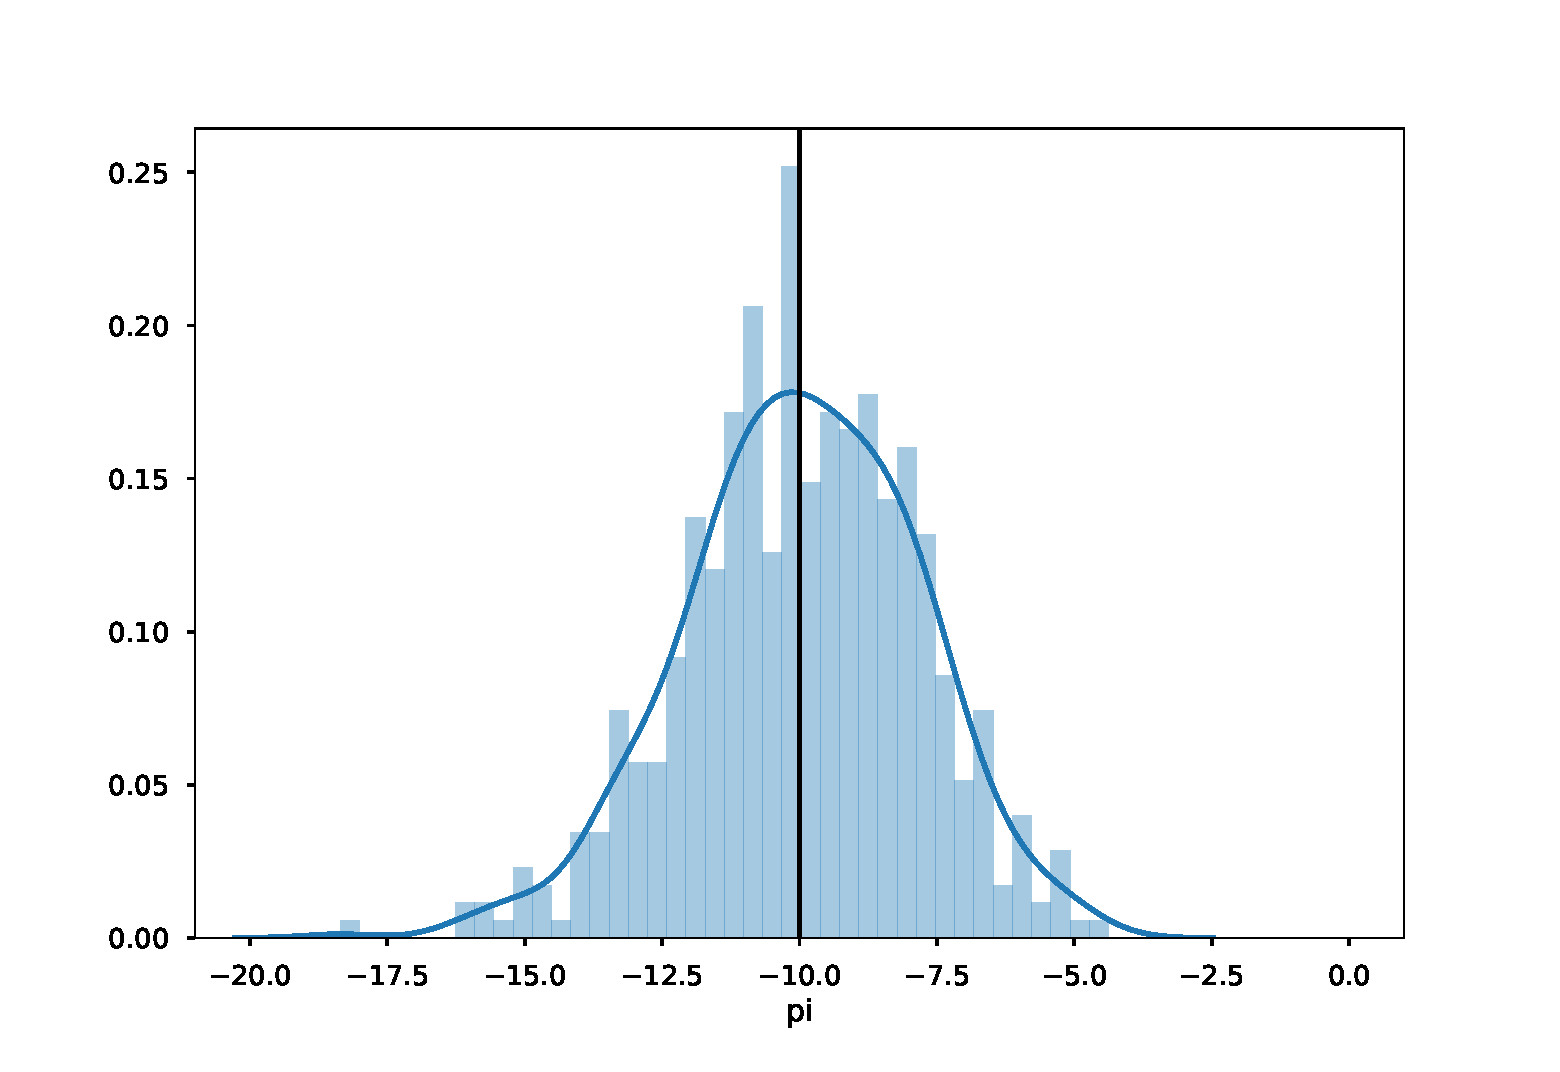
\includegraphics[width=\textwidth, height=\textwidth]{pi_est_500_-0_point_4.pdf}
  \end{subfigure}
  \begin{subfigure}[t]{.32\textwidth}
    \caption[phi = -0.10]{$\phi = -0.10$}
    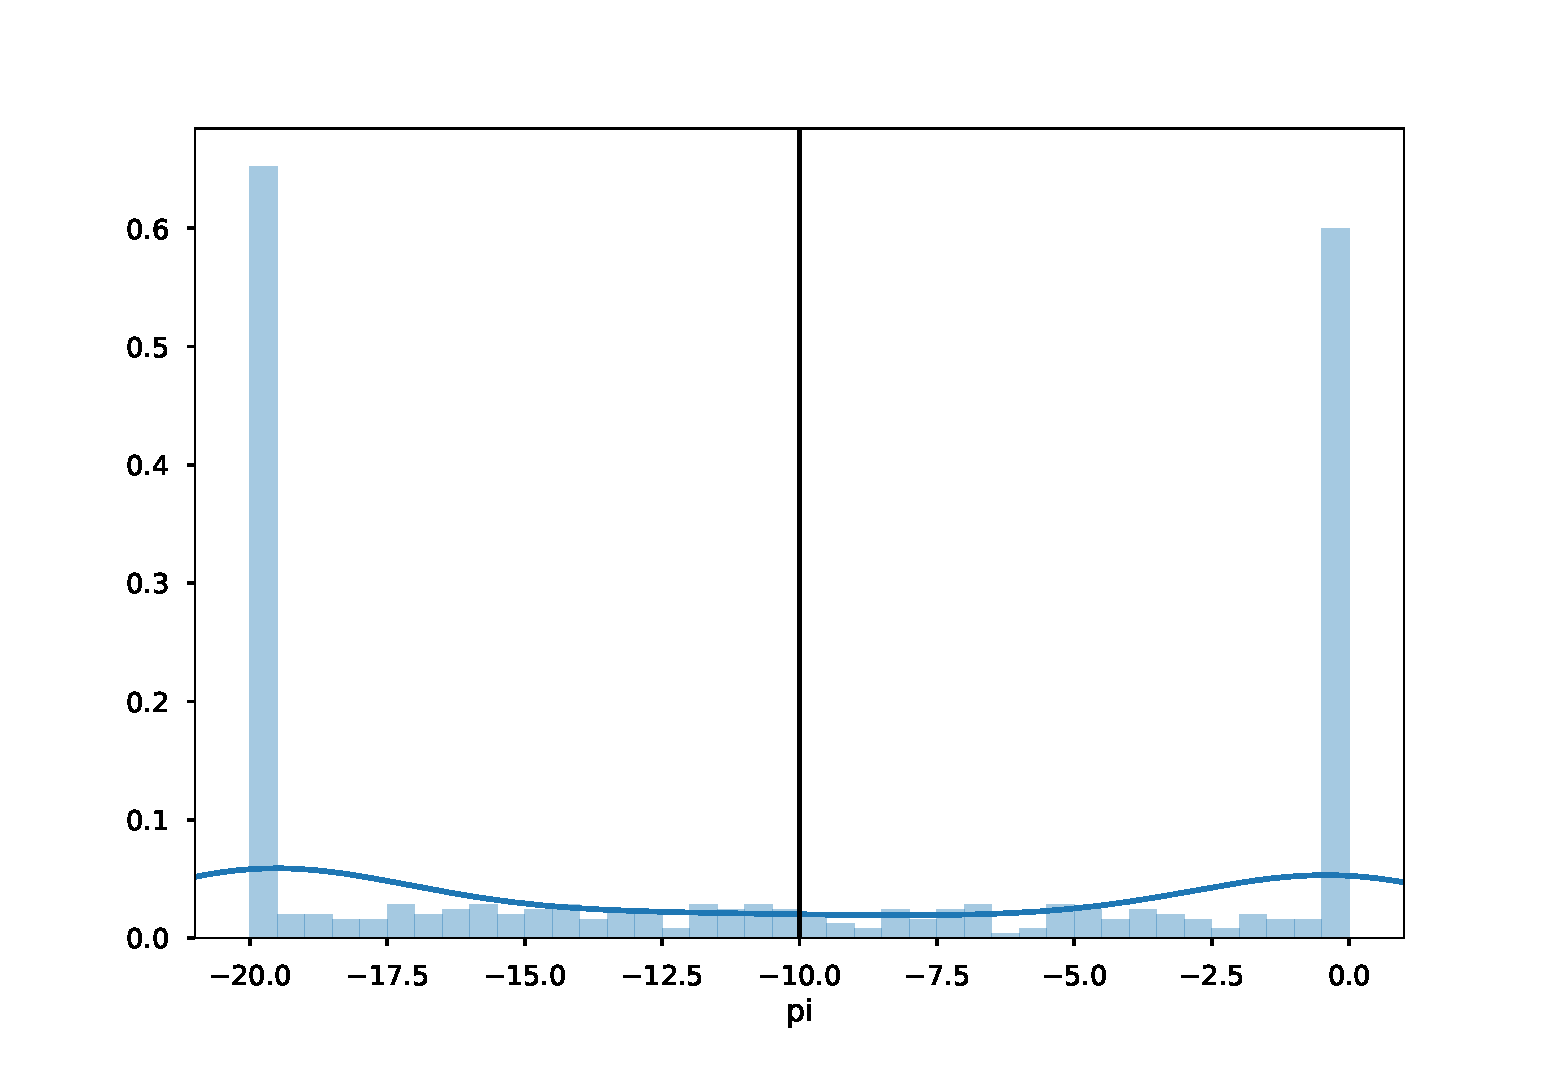
\includegraphics[width=\textwidth, height=\textwidth]{pi_est_500_-0_point_1.pdf}
  \end{subfigure}
  \begin{subfigure}[t]{.32\textwidth}
    \caption[phi = -0.01]{$\phi = -0.01$}
    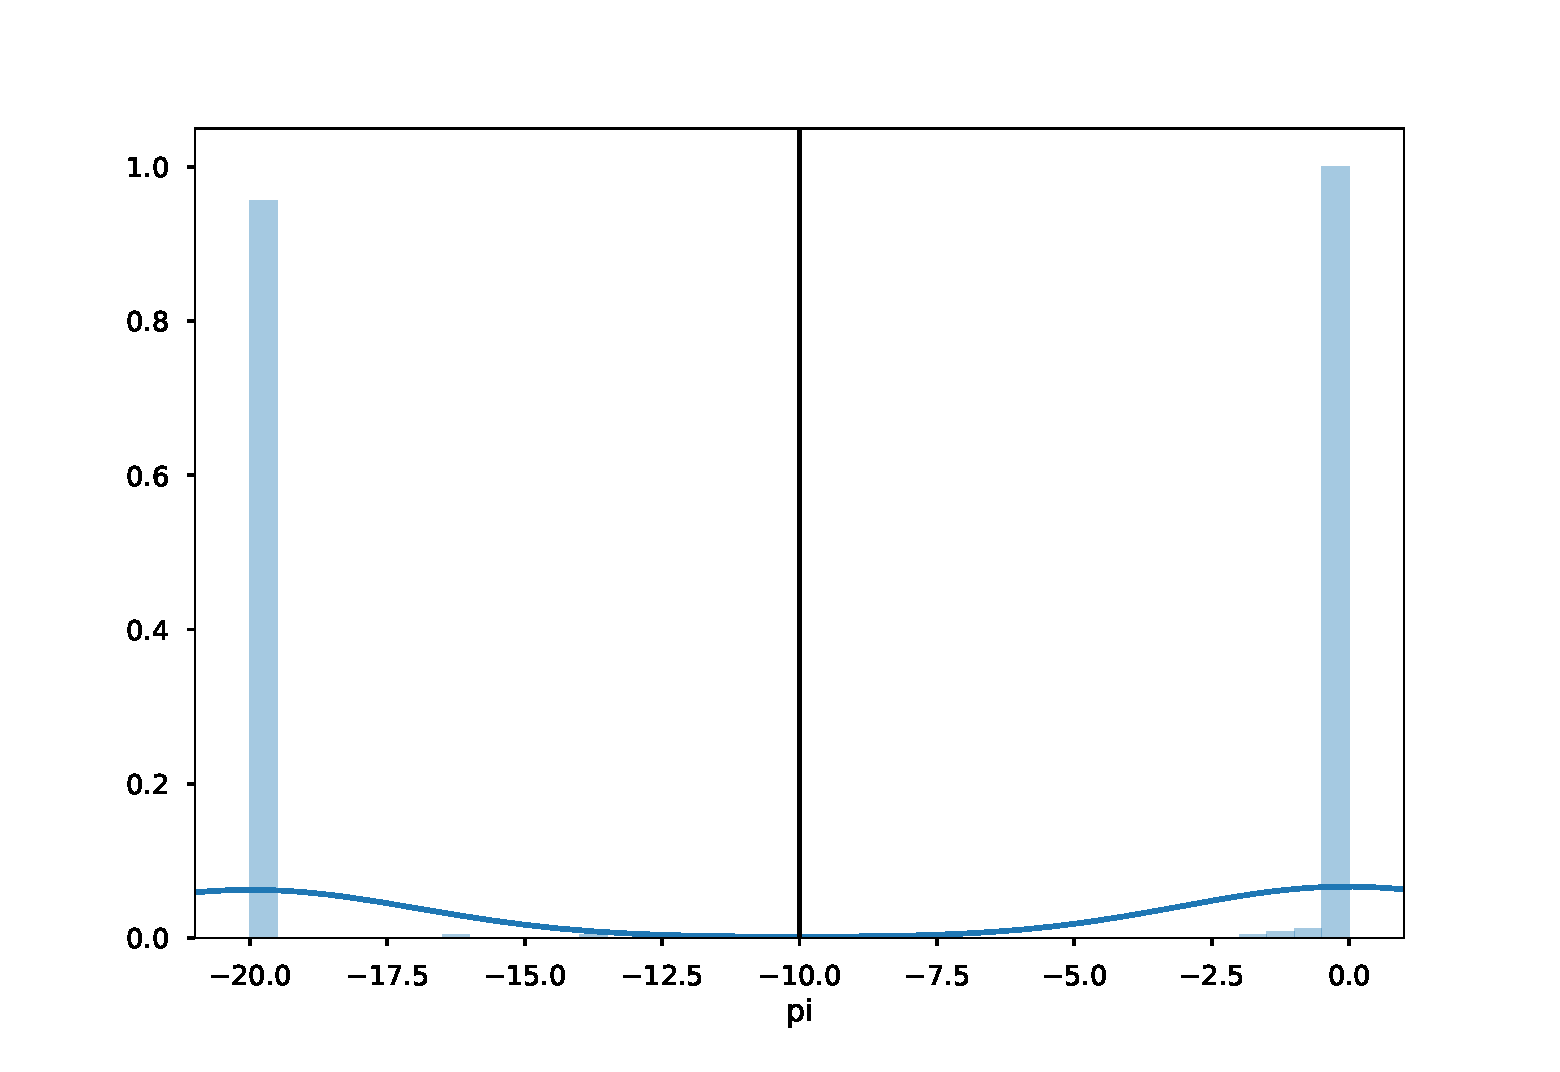
\includegraphics[width=\textwidth, height=\textwidth]{pi_est_500_-0_point_01.pdf}
  \end{subfigure}

\end{figure}

We now report the size of the $5{\percent}$ tests in finite-sample using the standard QLR test, the Anderson-Rubin (AR) test, and the conditional-QLR test proposed here.  The standard QLR test uses the same QLR statistic defined above, but the critical value is the $95{\percent}$ quantile of $\chi^2_{3}$. This is the correct critical value under strong identification only. Followiing \parencite{stock2000GMM}, the Anderson-Rubin statistic

\begin{equation}

AR = \widehat{g}(\lambda _{0})^{\prime }\widehat{\Sigma }(\lambda _{0},\lambda _{0})^{ -1}\widehat{g}(\lambda _{0}

\end{equation}

is roubst to weak identification. Because we have four link functions, the critical value for the AR test is the $95{\percent} quantile of  $\chi^2_{4}$.
%It should be valid in this context, but it is known to be very conservative in many applications. 

\begin{table}[htb]
 
  \centering
  \caption{Size in Finite Samples}
  \label{tbl:test_performance}

 \sisetup{
  round-mode=places,
  round-precision=3,
 }
 
 \begin{tabularx}{.75\textwidth}{X | *{3}{S} | *{3}{S}}
%
  \toprule
  $\phi$ & {QLR} & {AR} & {CLR} & {QLR} & {AR} & {CLR} \\
  \midrule
   \multicolumn{7}{c}{Parameter Values used by \textcite{han2018leverage}} \\
  \midrule
  & \multicolumn{3}{c}{$T$ = 3,700} & \multicolumn{3}{c}{$T$ = 37,000} \\
  \midrule
  -0.01  &  0.01400   & 0.00800   & 0.0580 & 0.01600  & 0.0100    & 0.04400   \\
  -0.10  &  0.0200    & 0.01000   & 0.0600 & 0.03200  & 0.0100    & 0.05400   \\
  -0.40  &  0.06200   & 0.01600   & 0.0760 & 0.0480   & 0.0200    & 0.05000   \\
%
  % \midrule
  %      \multicolumn{7}{c}{Parameters Estimated from the Data} \\
  % \midrule
  %     & \multicolumn{3}{c}{$T$ = 37000} & \multicolumn{3}{c}{$T$ = 3700} \\
  % \midrule
  % -0.01  & 0.0600  & 0.0300  & 0.06600                  \\ 
  % -0.10  &      &      &    & 0.084000  & 0.03600 & 0.09000 \\ 
  % -0.40  &      &      &    & 0.09200   & 0.06400 & 0.10400 \\
  \bottomrule

 \end{tabularx}

\end{table}

The finite-sample sizes of the three tests are reported in \cref{tbl:test_performance}. We start with the right column with the large sampel size. The $AR$-statistic is robust, but conservative.  The standard $QLR$-statistic appears to be conservative too. The $CLR$ test is robust and is the least conservative. In the left column with small sample size, the AR test is quite conservative. Both the CLR and the standard QLR tests tend to over-reject when $\phi = -0.40$.  This is likely because the variance of $r_{t+1}$ increases as $\phi$ increases. With the other parameters set as they are in \textcite{han2018leverage}, we need large samples to deal with the heteroskedasticity and non-Gaussianity in the data when $\phi$ is large in magnitude.


\section{Data and Empirical Results}\label{sec:empirical}

The two series we need to estimate the model are $r_{t+1}$ and $\sigma^2_{t+1}$, where $\sigma^2_{t+1}$ must be the volatility of $r_{t+1}$. %That is, we need the appropriately defined variance of $r_{t+1}$ to equal $\sigma^2_{t+1}$ in expectation as discussed in \cref{sec:leverage effect restrict}. 
Since this condition is automatically satisfied by the integrated volatility and daily return, we use high-frequency data to estimate $\sigma^2_{t+1}$ and use the associated daily return for $r_{t+1}$. 

For the market index, we use SPY (SPDR S\&P 500 ETF Trust), an exchange-traded fund that mimics the S\&P 500. This asset risk cannot be easily diversifiable.  We use the procedure \textcite{sangrey2018jumps} develops to estimate the integrated total volatility, which is the instantaneous expectation of the price variance, i.e., the time-derivative of the predictable quadratic variation. This measure reduces to the integrated diffusion volatility if prices have continuous paths. He shows in simulations that his method works well in the presence of market microstructure noise.

Since this paper only use one asset, and SPY is one of the most liquid assets traded, we can essentially choose the frequency at which we want to observe the underlying price. In order to balance market-microstructure noise, computational cost, and efficiency of the resultant estimators we sample at the \num{1} second frequency. The data starts in 2003 and ends in September 2017. Since the asset is only traded during business hours, this leads to \num{3713} days of data with an average of $\approx \num{24000}$ observations per day. We compute $r_{t+1}$ as the daily return from the open to close of the market because this is the interval over which we can estimate the volatility. Doing this avoids needing  to specify the relationship between overnight and intra-day returns. 

We preprocess the data using the pre-averaging approach as in \textcites{podolskij2009bipower, aitsahalia2012testing}. This procedure is known not to affect the consistency of the estimation procedure. The basic idea is to average the price over a small interval to remove the noise. %If we pick the rates at which we shrink the interval appropriately and thereby balance smoothing away the noise and allowing the volatility to vary intraday, the estimators are consistent.

\begin{figure}[htb]

  \centering
  \caption{S\&P 500 Volatility and Log-Return}


  \begin{subfigure}[t]{.54\textwidth}
    \label{fig:spy_dynamics}
    \caption{Time Series}
    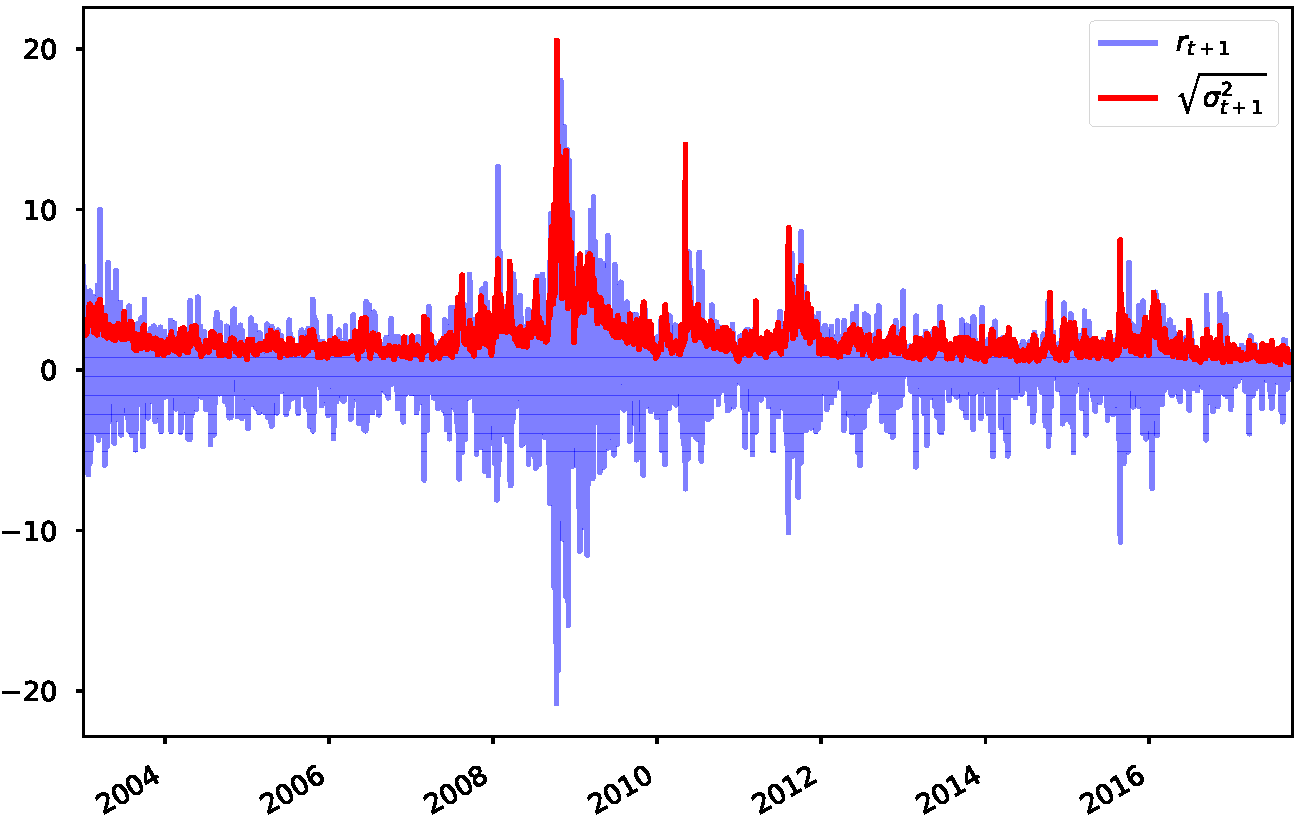
\includegraphics[width=\textwidth, height=.81\textwidth]{time_series.pdf}
  \end{subfigure}%
%
  \hfill
%
  \begin{subfigure}[t]{.44\textwidth}
    \label{fig:spy_static}
    \caption{Joint Distribution}
    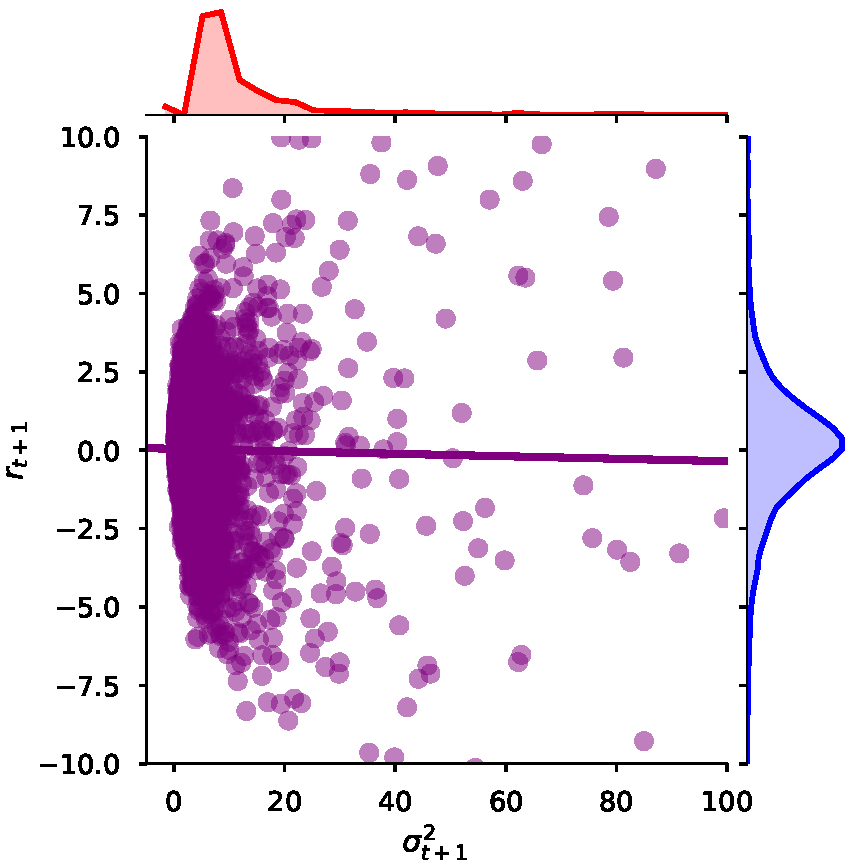
\includegraphics[width=\textwidth, height=\textwidth]{joint_dist.pdf}
  \end{subfigure}
\end{figure}


To see how the data move over time, we plot their time series in  \cref{fig:spy_dynamics}.  We also plot the joint unconditional distribution in \cref{fig:spy_static} to see the static relationship between the two series. The volatility has a long-right tail, for a typical gamma-type distribution, and the returns have a bell-shaped distribution. They are also slightly negative correlated as can be seen by the regression line in the joint plot.

We also report a series of summary statistics. The volatility and returns are weakly negatively correlated, corroborating the work by \textcites{bandi2012timevarying, aitsahalia2013leverage}. 

\begin{table}[htb]

  \centering
  \caption{Summary Statistics}
  \label{tbl:summary_stats}


  \sisetup{
   table-align-text-pre=false,
   table-align-text-post=false,
   round-mode=places,
   round-precision=2,
   table-space-text-pre=\lbrack,
   table-space-text-post=\rbrack,
  }

  \begin{tabularx}{.5\textwidth}{X | S S}
    \toprule
    & {$r_{t+1}$} & {$\sigma^2_{t+1}$} \\
    \midrule
      Mean & 0.023421 & 5.621287 \\
      \rowcolor{gray!20}
      Standard Deviation & 2.350165 & 14.458446\\
      Skewness & -0.312 & 12.209 \\
      \rowcolor{gray!20}
      Kurtosis & 10.055 & 240.401 \\
      Correlation & \multicolumn{2}{c}{\num{-0.024379}} \\
    \bottomrule
  \end{tabularx}

\end{table}


We now report the estimates and confidence intervals for the reduced-form parameters. We only report the reduced-form parameters that are true determinants of the model, i.e., they are necessary to simulate the model. The other reduced-form parameters are known functions of these parameters and the structural parameters. These parameters have no economic meaning and are only useful in the estimation procedure. The confidence intervals reported here use the Gaussian limiting theory, ($\pm 1.96$ standard errors) but we truncate at the edge of the parameter space if necessary. Although, these reduced-form parameters can be estimated directly from the data, disentangling $c$ and $\delta$ is difficult, and so the estimation procedure responds appropriately by reporting relatively large standard errors. 


\begin{table}[htb]
  \caption{Reduced-Form Parameter Estimates} 
  \label{tbl:reduced_form_parameters}

  \centering
  \sisetup{
    table-align-text-pre=false,
    table-align-text-post=false,
    round-mode=places,
    table-alignment=center,
  }

  \begin{tabularx}{.5\textwidth}{X | S >{{(}} S[table-space-text-pre={(}] <{{,\,}}
    S[table-space-text-pre={\hspace{-1cm}}] <{{)}}}
%
    \toprule
    & {Point Estimate} & \multicolumn{2}{c}{Confidence Interval} \\
    \midrule
    $c$     & 3.112013 & 0.00 & 7.379227 \\
    % $c$     & 3.112013 & -1.155201 & 7.379227 \\
    \rowcolor{gray!20}
    $\delta$  & 0.2678579 & 0.00 & 3.007632 \\
    % $\delta$  & 0.2678579 & -2.471916 & 3.007632 \\
    $\rho$   & 0.807506 & 0.402264 & 1.00 \\
    % $\rho$   & 0.807506 & 0.402264 & 1.212748 \\
    \bottomrule 
  \end{tabularx}
\end{table}


We are interested in not just the reduced-form parameters. We also want estimates for $\phi$ and the risk prices. Since $\phi < 0$, our estimator is consistent and the point estimate is a meaningful number. We report the \SI{95}{\percent} confidence intervals by computing the joint confidence interval above, and then projecting down to the each of the components.


\begin{table}[htb]
  \caption{Structural Parameter Estimates} 
  \label{tbl:structural_param_estimates}

  \centering
  \sisetup{
    table-align-text-pre=false,
    table-align-text-post=false,
    round-mode=places,
    round-precision=2,
    table-alignment=center,
  }

  \begin{tabularx}{.5\textwidth}{X | S >{{(}} S[table-space-text-pre={(}] <{{,\,}}
    S[table-space-text-pre={\hspace{-1cm}}] <{{)}}}
%
    \toprule
    & {Point Estimate} & \multicolumn{2}{c}{Confidence Interval} \\
    \midrule
    $\phi$   & -0.302417 & 0.30 & -0.20 \\
    \rowcolor{gray!20}
    $\pi$    & -0.115097 & -0.2500 & 0.0 \\
    $\theta$   & 0.516140 & 0.20 & 0.6 \\
    \bottomrule 
  \end{tabularx}
\end{table}

The parameters in \cref{tbl:structural_param_estimates} have a few notable features. First, we can reject $\phi = 0$ at the \SI{95}{\percent} level. We cannot, however, reject $\pi = 0$. Interestingly, the values for $\phi, \pi$, and $\theta$ reported by \textcite{han2018leverage} lie outside our confidence interval for each of the parameters. They calibrate $\pi = -10$ and then estimate the remaining parameters. 

%Since their calibration of $\pi$ is badly misspecified, their resulting estimates for $\theta$ is biased in finite sample. Conversely, our estimates do not lie outside their confidence intervals. Even though our estimation procedure for the parameters individually is conservative, as induced by the projection above, our estimates are still more precise in practice. This difference is likely a result of our estimation procedure more effectively using the information about the various parameters jointly, which their partially calibrated model is incapable of doing.

The main issue with the confidence interval in \cref{tbl:structural_param_estimates} is that they are conservative because we go from joint inference to sub-vector inference by using an inherently conservative projection-based procedure. Plots of confidence region in three dimensions are not particularly easy to understand, and so we report a joint confidence set for the two prices. %This analysis is still conservative as we project out $\phi$, but not as conservative as the univariate analysis.


\begin{figure}[htb]

  \centering
  \caption{Confidence Set for Risk Prices}
  \label{fig:confidence_region}

  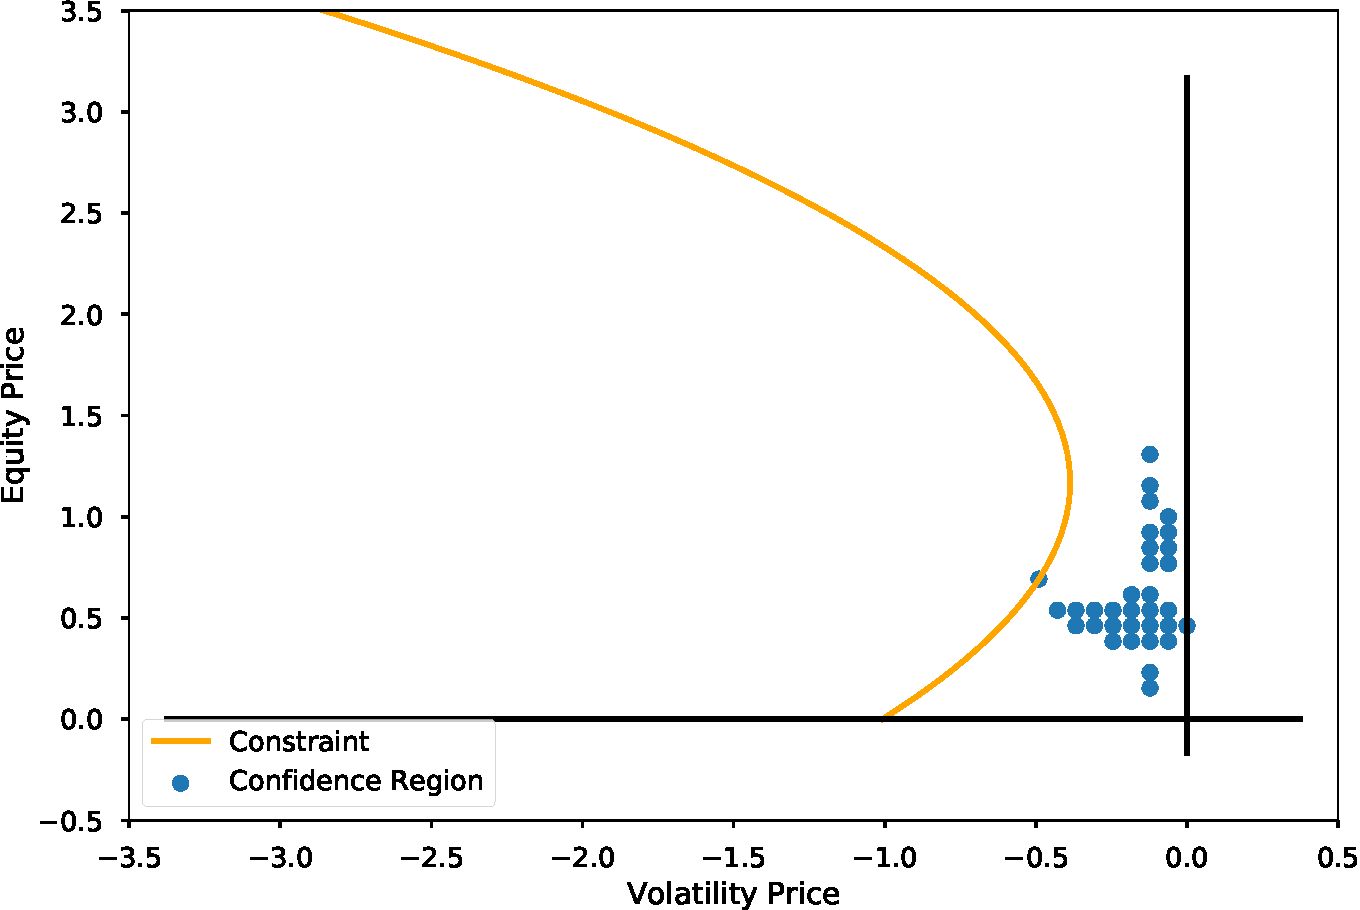
\includegraphics[width=.5\textwidth]{confidence_region.pdf}
\end{figure}

The confidence set is approximately rectangular, so the projection inference we reported in \cref{tbl:structural_param_estimates} does not over cover much. It is worth noting that confidence set does not have to be connected. 

%Furthermore, since we plot the constraint on the potential value of the parameters, we can see that except for $\pi < 0$, the other constraints do not bind in practice. The joint likelihood appears to be multi-modal but since the asymptotic distribution is not Gaussian, this not surprising.



\section{Conclusion}\label{sec:conclusion}

%TODO
%we have reduce the overlap with the abstract and intro. I will think about it.

In structural stochastic volatility models such as the one developed here, changes in the volatility affect returns through two channels. First, the investor's willingness to tolerate high volatility in order to get high expected returns as measured by the price of market risk. Standard economic models imply there is a static trade-off between risk and expected return. Consequently, when the risk changes the expected return must change to restore equilibrium. However, investors may also be directly averse to changes in future volatility, and the empirical evidence shows that they are. \Textcite{han2018leverage} shows that we can disentangle these two channels through their differing relationships to the leverage effect. However, estimating the leverage effect is quite tricky, \parencite{aitsahalia2013leverage}. This difficulty poses a subtle identification problem that invalidates standard inference. When the data's signal-to-noise ratio is small, as it is here, standard tests and confidence intervals provide misleading results. We adopt the discrete-time exponentially-affine of \textcite{han2018leverage} and adapt weak identification methods to this framework to ensure that the resulting confidence intervals are uniformly valid.

In particular, we develop a minimum distance criterion that links the market risk price, the volatility risk price, and the leverage effect to some well-behaved reduced-form parameters that govern the return and volatility's joint distribution. We do this by adapting the conditional quasi-likelihood ratio test (CLR) \textcite{andrews2016conditional} develop in a GMM framework to a minimum distance framework. The resulting CLR test is uniformly valid. We invert this test to derive a robust confidence set. We then apply this methodology to data on the S\&P 500 and show that the market risk price lies between \num{0.20} and \num{0.60} yearly percentage points, and the volatility risk price lies between \num{-0.20} and \num{0.00} yearly percentage points. These estimates are both substantially smaller in magnitude than the values chosen by \textcite{han2018leverage}.


\clearpage

\addcontentsline{toc}{section}{References}
\printbibliography

\begin{appendices}

\section{Proofs}\label{sec:proofs}


\subsection{\texorpdfstring{Proof of \cref{Lemma m0 and m1}}{Proof of Lemma 1}}

\begin{proof}
For the risk free asset, $ r_{t+1}=0.$ 
Therefore, we have
%
\begin{align*}
    1 &= E\left[ \exp \left( m_{0}+m_{1}\sigma _{t}^{2}-\pi \sigma _{t+1}^{2}-\theta r_{t+1}\right) \mvert \F_{t}\right]  \\
%
    &= \exp (m_{0}+m_{1}\sigma _{t})E\left[ \exp \left( -\pi \sigma _{t+1}^{2}\right) E\left[ \exp \left( -\theta r_{t+1}\right) \mvert \F _{t},\sigma _{t+1}^{2}\right] \mvert \F_{t}\right]  \\
%
    &= \exp (m_{0}-E\left( \theta \right) +m_{1}\sigma _{t}-D\left( \theta \right) \sigma _{t}^{2})E\left[ \exp \left( -\pi \sigma _{t+1}^{2}-C\left( \theta \right) \sigma _{t+1}^{2}\right) \mvert \F_{t}\right]  \\
%
    &= \exp (m_{0}-E\left( \theta \right) +m_{1}\sigma _{t}-D\left( \theta \right) \sigma _{t}^{2}-A\left( \pi +C\left( \theta \right) \right) \sigma _{t}^{2}-B\left( \pi +C\left( \theta \right) \right) ),
%
\end{align*}
%
where the first equality follows from the pricing equation, the second equality follows from the law of iterated expectations, the third equation uses the Laplace transform for $r_{t+1}$ in \cref{eqn:return_laplace_transform}, and the last equality follows from the Laplace transform for $\sigma _{t+1}^{2}$ in \cref{eqn:vol_laplace_transform}. 
Since $M_{t,t+1}$ must integrate to $1$, the constant term and coefficient for $\sigma_{t}^{2}$ must equal 0, which gives the claimed result for $m_{0}$ and $m_{1}$.

We can apply the same argument above to any asset $r_{t+1}$. This gives the same result, except $\theta$ is replaced by $\theta -1$ throughout. 
This implies that the two equalities for $m_{0}$ and $m_{1}$ also hold with $\theta $ replaced by $\theta -1$. 
Therefore, 
%
\begin{align*}
    E(\theta -1)+B\left( C\left( \theta -1\right) +\pi \right)  
%
    &= E(\theta)+B\left( C\left( \theta \right) +\pi \right) , \\
%
    D\left( \theta -1\right) +A\left( C\left( \theta -1\right) +\pi \right) 
%
    &= D\left( \theta \right) +A\left( C\left( \theta \right) +\pi \right).
\end{align*}
%
The claimed results for $\gamma $ and $\beta $ follow from $\gamma = \E(\theta)-E(\theta -1)$ and $\beta =D(\theta )-D(\theta -1)$ under the linear specification of $E(x)=\gamma x$ and $D(x)=\beta x$.

\end{proof}

\subsection{\texorpdfstring{Proof of \cref{Lemma Reduce}}{Proof of Lemma 2}}

\begin{proof}

    Under the assumption that (i) $ \mathbb{E(}z_{t}z_{t}^{\prime })$ has the smallest eigenvalue bounded away from 0 and (ii) $c>\varepsilon $ and $\delta >\varepsilon $ for some $ \varepsilon >0,$ we not only have $\omega _{10}$ as an uniquely minimizer of $||\mathbb{E}[h_{t}(\omega _{1})]||$ but also have a uniform positive lower bound for $\norm{\E[h_{t}(\omega _{1})]}$ for $\norm{\omega _{1}-\omega _{10}} \geq \varepsilon$. Thus, consistency of $\widehat{\omega }_{1}$ follows from standard arguments for the consistency of a GMM estimator under an uniform convergence of the criterion under \cref{assump:R} (1) and (2).

Let $\overline{h}(\omega _{1})=T^{-1}\sum_{t=1}^{T}h_{t}(\omega _{1})$ and $ \overline{H}(\omega )=T^{-1}\sum_{t=1}^{T}H_{t}(\omega _{1}).$ By construction, the estimator satisfies the first order condition
%
\begin{align}
    0 &= 
    \begin{pmatrix} 
        \overline{H}(\widehat{\omega }_{1})^{\prime }\widehat{V}_{1}^{-1}\overline{h} (\widehat{\omega }_{1}) \\ 
%
        T^{-1}\sum_{T=1}^{T}x_{t}(y_{t}-x_{t}^{\prime }\widehat{\omega }_{2}) \\ 
%
        \widehat{\omega }_{3}-T^{-1}\sum_{t=1}^{T}\left( y_{t}-\widehat{y} _{t}\right) ^{2} 
    \end{pmatrix} \nonumber \\ 
%
    &= 
%
    \begin{pmatrix}
%
        \overline{H}(\widehat{\omega }_{1})^{\prime }\widehat{V}_{1}^{-1}\overline{h} (\omega _{10})+\overline{H}(\widehat{\omega }_{1})^{\prime }\widehat{V} _{1}^{-1}\overline{H}(\widetilde{\omega }_{1})(\widehat{\omega }_{1}-\omega
_{10}) \\ 
%
        T^{-1}\sum_{t=1}^{T}x_{t}(y_{t}-x_{t}^{\prime }\omega _{20})-T^{-1}\sum_{t=1}^{T}x_{t}x_{t}^{\prime }\left( \widehat{\omega } _{2}-\omega _{20}\right) \\ 
%
        \left( \widehat{\omega }_{3}-\omega _{3}\right) +\omega _{3}-T^{-1}\sum_{t=1}^{T}\left( y_{t}-x_{t}\widehat{\omega }_{2}\right) ^{2}
    \end{pmatrix},
%
  \label{L-R-1}
\end{align}
%
where the second equality follows from a mean value expansion of $\overline{h }(\widehat{\omega }_{1})$ around $\omega _{10},$ with $\widetilde{\omega } _{1}$ between $\omega _{10}$ and $\widehat{\omega }_{1}$. 
Let
%
\begin{equation}
%
    \widetilde{\mathcal{B}} = \diag\left\lbrace[\overline{H}(\widehat{\omega }_{1})^{\prime } \widehat{V}_{1}^{-1}\overline{H}(\widetilde{\omega }_{1})]^{-1}\overline{H}( \widehat{\omega }_{1})^{\prime }\widehat{V}_{1}^{-1},[T^{-1} \sum_{t=1}^{T}x_{t}x_{t}^{\prime }]^{-1},1\right\rbrace.  
%
\end{equation}
%
Then \cref{L-R-1} implies that 
%
\begin{align}
    T^{1/2}\left( \widehat{\omega }-\omega \right) 
%    
    &= \widetilde{\mathcal{B}} \cdot T^{-1/2}\sum_{t=1}^{T} 
%
    \begin{pmatrix}
        -h_{t}(\omega _{10}) \\ 
%
        x_{t}(y_{t}-x_{t}^{\prime }\omega _{20}) \\ 
%
        \left( y_{t}-x_{t}\widehat{\omega }_{2}\right) ^{2}-\omega _{3}%
    \end{pmatrix}  \nonumber \\
%
    &=
%
    \widetilde{\mathcal{B}}\cdot T^{-1/2}\sum_{t=1}^{T} 
%
    \begin{pmatrix}
        -h_{t}(\omega _{10}) \\ 
%
        x_{t}(y_{t}-x_{t}^{\prime }\omega _{20}) \\ 
%
        \left( y_{t}-x_{t}^{\prime }\omega _{20}\right) ^{2}-\E\left[\left( y_{t}-x_{t}^{\prime }\omega _{20}\right)^{2}\right]%
%
    \end{pmatrix}%
%
    +
%
    \begin{pmatrix}
        0 \\ 
        0 \\ 
        \varepsilon_{T}
    \end{pmatrix},
%
    \label{L-R-2}
%
\end{align}%
%
where the second equality uses $\omega _{3}=\E[\left( y_{t}-x_{t}^{\prime }\omega _{20}\right) ^{2}]$ by definition and 
%
\begin{align}
    \varepsilon _{T} 
%
    &= T^{-1/2}\sum_{t=1}^{T}\left[ \left( y_{t}-x_{t}^{\prime } \widehat{\omega }_{2}\right) ^{2}-\left( y_{t}-x_{t}^{\prime }\omega _{20}\right) ^{2}\right]  \nonumber \\
%
    &= 2T^{-1}\sum_{t=1}^{T}\left( y_{t}-x_{t}^{\prime }\omega _{20}\right) x_{t}^{\prime }\left[ T^{1/2}\left( \widehat{\omega }_{2}-\omega _{20}\right) \right] +o_{p}(1)  \nonumber \\
%
    &= o_{p}(1)  
%
    \label{L-R-3}
\end{align}
%
because $T^{-1}\sum_{t=1}^{T}\left( y_{t}-x_{t}^{\prime }\omega _{20}\right) x_{t}^{\prime }\rightarrow _{p}0$ and $T^{1/2}(\widehat{\omega }_{2}-\omega _{20})=O_{p}(1)$ following \cref{assump:R}. 
In addition, 
%
\begin{equation}
    \widetilde{\mathcal{B}}\rightarrow _{p}\mathcal{B}  
    \label{L-R-4}
\end{equation}%
%
following from the consistency of $\widehat{\omega}_{1}$ and \cref{assump:R}.  Finally, the desirable result follows from \cref{L-R-2}--\cref{L-R-4} and \cref{assump:R}.  The consistency of $\widehat{\Omega }$ follows from the consistency of $\widehat{\mathcal{B}}$ and $\widehat{V}$. 

\end{proof}

\subsection{\texorpdfstring{Proof of \cref{Lemma CS}}{Proof of Theorem 3}}

\begin{proof}

We obtain this result by applying \textcite[Theorem 1]{andrews2016conditional}. 
We now verify Assumptions 1-3 in \textcite{andrews2016conditional}. 
To show weak convergence $\eta _{T}(\cdot )$ to $\eta (\cdot )$ uniformly over $\mathcal{P}$, note that by a second-order Taylor expansion,
%
\begin{align}
    \eta _{T}(\lambda) 
%
    &\coloneqq T^{1/2}\left[ \widehat{g}(\lambda )-g_{0}(\lambda ) \right] = G_{0}(\lambda )\Omega ^{1/2}\xi _{T}+\delta _{T},\text{ where} \nonumber \\
%
    \xi _{T} 
    &= \Omega ^{-1/2}T^{1/2}\left( \widehat{\omega }-\omega _{0}\right), \text{ and } 
%
    \delta _{T} =\left( G(\lambda ,  \widetilde{\omega })-G(\lambda, \omega _{0})\right) T^{1/2}(\widehat{\omega }-\omega _{0})
%
\end{align}%
%
and $\widetilde{\omega }$ is between $\widehat{\omega }$ and $\omega_{0}$.
%
Because $\norm{G(\lambda ,\widetilde{\omega })-G(\lambda ,\omega _{0})} \leq C \norm{\widetilde{\omega }-\omega_{0}}$, $\delta _{T}=o_{p}(1)$ uniformly over $ \mathcal{P}$ following Lemma \cref{Lemma Reduce}. 
To show $G_{0}(\lambda)\Omega ^{1/2}\xi _{T}$ weakly converges to $\eta (\cdot ),$ it is sufficient to show (i) the pointwise convergence%
%
\begin{equation}
% 
    \begin{pmatrix}
        G_{0}(\lambda _{1})\Omega ^{1/2}\xi _{T} \\ 
        G_{0}(\lambda _{2})\Omega ^{1/2}\xi _{T}%
    \end{pmatrix}%
%
    \rightarrow _{d}( 
%
    \begin{pmatrix}
        \eta (\lambda _{1}) \\ 
        \eta (\lambda _{2})%
    \end{pmatrix},
%
\end{equation}%
%
which follows from \cref{Lemma Reduce}, and (ii) the stochastic equicontinuity condition, i.e., for every $\varepsilon >0$ and $\xi >0,$ there exists a $\delta >0$ such that
%
\begin{equation}
    \underset{T\rightarrow \infty }{\lim\sup }\Pr \left( \underset{P\in \mathcal{P}}{\sup }\underset{\norm{\lambda _{1}-\lambda _{2}}\leq \delta }{\sup }\norm*{G_{0}(\lambda _{1})\Omega ^{1/2}\xi _{T}-G_{0}(\lambda
    _{2})\Omega ^{1/2}\xi _{T}} >\varepsilon \right) < \xi.
\end{equation}%
%
For some $C < \infty$, we have $\norm{G_{0}(\lambda _{1})-G(\lambda _{2})} \leq C \norm{\lambda _{1}-\lambda _{2}}$ under a uniform bound for the derivative in \cref{assump:S}, and we have $\norm{\Omega ^{1/2}} \leq C$ under \cref{assump:R} because $F$ and $V$ both have bounded largest eigenvalue. 
Thus,
%
\begin{align}
    &\phantom{=} \underset{T\rightarrow \infty }{\lim \sup }\Pr\left( \underset{P\in \mathcal{P}}{\sup }\underset{\norm{\lambda _{1}-\lambda _{2}}\leq \delta }{\sup }\norm*{ G_{0}(\lambda _{1})\Omega ^{1/2}\xi _{T}-G_{0}(\lambda _{2})\Omega ^{1/2}\xi _{T}} > \varepsilon \right)  \nonumber \\
%
    &\leq \underset{T\rightarrow \infty }{\lim \sup }\Pr \left( C^{2}\underset{ P\in \mathcal{P}}{\sup }\left \Vert \xi _{T}\right \Vert >\frac{\varepsilon }{\delta }\right). 
%
    \label{EC}
\end{align}
%
Because $\xi _{T}=O_{p}(1)$ uniformly over $P\in \mathcal{P},$ there exists $ \delta $ such that $\varepsilon /\delta $ is large enough to make the right hand side of the inequality in \cref{EC} smaller than $\xi$.

Assumptions 2 and 3 of \textcite[Theorem 1]{andrews2016conditional} follow from \cref{assump:R}. 
\end{proof}


\end{appendices}

\end{document}


